\chapter{Problema 2}

\section{Little Bishops}

Un alfil es una pieza utilizada en el juego de ajedrez el cual es jugado en una tabla con grillas cuadradas. Un alfil puede moverse solamente de forma diagonal desde su posici�n actual, y dos alfiles se atacan si uno de ellos est� en el camino del otro. En la siguiente figura, los cuadrados negros representan los lugares alcanzables por el alfil $B_1$ desde su posici�n actual. La figura tambi�n muestra que los alfiles $B_1$ y $B_2$ est�n en posiciones de ataque, pero $B_1$ y $B_3$ no. $B_2$ y $B_3$ tampoco se atacan.

\begin{figure}[H]
\centering
\label{ej2_tableroEnunciado}
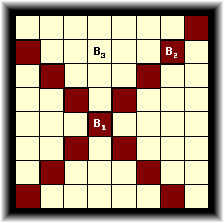
\includegraphics[scale=0.5]{./graficos/ej2/tableroEnunciado.jpg}
\end{figure}

Ahora, dados dos n�meros \textbf{n} y \textbf{k}, su deber es determinar la cantidad de formas en que uno puede ubicar $k$ alfiles en un tablero de ajedrez de $n � n$, de forma tal que ningun par de ellos se atacan.
 
\textbf{Entrada:}

El archivo de entrada puede contener m�ltiples casos de test. Cada test ocupa una l�nea en el archivo de entrada y contiene dos enteros \textbf{n} $(1 \le n \le 8)$ y \textbf{k} $(0 \le k \le n^2)$. 

Un caso de test que contiene dos ceros para n y k finaliza la entrada y no necesitar� procesar esta particular entrada.
 
\textbf{Salida:}

Para cada caso de test en la entrada imprimir una l�nea conteniendo el n�mero total de formas en la cual uno puede ubicar la cantidad de alfiles dada en un tablero de ajedrez del tama�o dado tal que ningun par de ellos se atacan. Puede asumir que este n�mero ser� menor a $10^{15}$.

\textbf{Url:}

\href{http://uva.onlinejudge.org/index.php?option=com\_onlinejudge\&Itemid=8\&category=10\&page=show\_problem\&problem=802}{Problema de Little Bishops}

\subsection{Soluci�n}
